% Selected DSN2027 manuscript; evidence and release provenance are archived separately.
\documentclass[conference,10pt]{IEEEtran}
\usepackage[T1]{fontenc}
\usepackage{cite,amsmath,amssymb,amsthm}
\usepackage{booktabs,array,multirow,graphicx}
\usepackage{url,microtype}
\usepackage[hidelinks]{hyperref}
\newtheorem{definition}{Definition}
\newtheorem{proposition}{Proposition}
\begin{document}
\title{RevTrace: Preserving Valid Progress across Trusted Feedback Revisions}
\author{\IEEEauthorblockN{Anonymous submission}\IEEEauthorblockA{Regular paper}}
\maketitle
\begin{abstract}
Trusted feedback can invalidate speculation while leaving computation and
delivered progress usable. RevTrace coordinates full-input eligibility,
protected selection, and whole-hypothesis consumption. Frozen inputs
confirm owned calls; a separate dependency witness governs visible views.
Native calls retain original correction even when their own next
predictions are wrong. A selected-trace refinement argument connects
durable facts and recovery to the protected program. In a predeclared
24-speaker stratum, computation retention alone increases frontier
withdrawals from 12 to 17; joint coordination produces zero and adds
26.645 seconds of deadline credit over 714.110 seconds offered. A matched
32-run native comparison preserves original histories: the final protocol
delivers 65.822 of 66.340 deadline-credited seconds and passes both
whole-run deadlines in six of eight trials, versus none for conservative
execution. Fault and sustained-state tests expose recovery, quality,
and resource boundaries.
\end{abstract}
\begin{IEEEkeywords}
dependable inference, feedback state, incremental computation, speculative execution, streaming ASR
\end{IEEEkeywords}
\section{Introduction}\label{sec:intro}
Feedback-driven speech recognition uses generated text as input to later
inference. A trusted correction can change that input, invalidating some
speculative work while leaving other work usable. A dependable service
must distinguish these cases and preserve useful delivered progress while
the trusted path catches up.

Computation retention alone can exacerbate this mismatch. In our
predeclared Qwen evaluation on three new eight-speaker cohorts, retaining
valid computation improved timely delivery but increased observed
audio-frontier withdrawals from 12 to 17 when the Consumer still installed
snapshots. Retaining the computation and its compatible whole view together
produced zero frontier withdrawals in that stratum. The issue is how valid
work becomes sustained service across a trusted update.

One actual two-second interval illustrates the loss. Its complete
hypothesis reached the Consumer at 1.444~s, meeting the two-second display
deadline. At 1.544~s, a new certified root replaced it with a shorter
snapshot, although the whole hypothesis retained a valid dependency path.
It remained absent at the original deadline and returned with identical
text at 3.720~s through certified delivery, within the eight-second deadline.
Both first-delivery obligations were met, yet 37 newly displayed characters,
including spaces, disappeared for 2.176~s. This is lost interval coverage
under a compatible update, independently of transcription correctness.

\begin{figure*}[t]
\centering
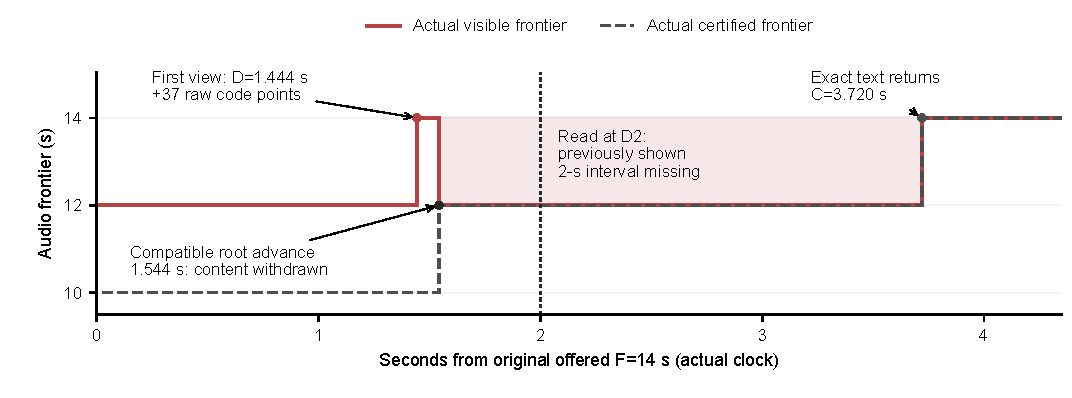
\includegraphics[width=\textwidth]{figures/timely_full_interval_case.pdf}
\caption{An actual computation-only interval meets first-display D2 and
certified-delivery C8, yet loses its phrase for 2.176~s under a compatible
update. The dotted line samples the original D2 read point. This case
comes from c16, whose whole-run D2 P99 fails; it is neither a paired
counterfactual nor a natural-prevalence estimate.}
\label{fig:continuity_case}
\end{figure*}

Incremental dialogue distinguishes active and committed information and
propagates revocation~\cite{schlangen2011incremental}; incremental
computation reuses dependencies and stable identities
\cite{hammer2014adapton,hammer2015names,mcsherry2013differential}.
SSBD combines old draft reuse with display-only masking in
re-translation~\cite{zeng2026ssbd}, and PredGen speculates on downstream
responses during evolving speech~\cite{li2025predgen}. RevTrace applies
these ideas to a protected task whose original selection recursively
supplies later ASR inputs. Separate sufficient guards determine whether
old computation remains eligible and whether installing a root preserves
the Consumer's current whole hypothesis. Original selection retains
write authority and incompatible revisions remain necessary.

Complete frozen inputs supply the eligibility witness. The core runtime
checks recorded continuation paths; a native correction pipeline confirms
inputs of already executing full calls. A call can have a valid input
even when its own predicted next state is wrong. The Consumer independently
checks its visible whole view. Selected facts, provisional views, and
physical execution retain distinct identities through message rejection,
durable selection, and recovery.

This paper makes three contributions:
\begin{itemize}
\item A feedback-state contract with separate executable witnesses for
  computation eligibility and whole-view retention across selected roots.
  Complete inputs, output dependencies, and execution identities determine
  what survives; a version change alone does not.
\item A coordinator that preserves the original selected transition relation
  while retaining compatible computation and views. Its conditional
  guarantees distinguish provisional delivery, durable selection, and
  physical ownership, including supported process failures.
\item Actual service evidence with the selected task fixed: factorial
  controls expose computation-only withdrawal, native correction tests
  input-confirmed full calls, and fault and sustained-state trials test
  the coordinator's boundaries and costs.
\end{itemize}

The headline joint design adds 26.645~s of dual-deadline credit over
714.110~s offered without changing certified histories. A separate 48-run
study retains the negative intermediate-load result and distinguishes
subsequent availability from first delivery. A matched native comparison
holds inputs, models and conditions fixed across the earlier and final
implementations. The final protocol raises credit from 30.0 to 65.822
of 66.340~s offered and whole-run passes from zero to six of eight,
retaining its two EOS misses.

\section{Feedback Contract}\label{sec:contract}
\subsection{Feedback creates an execution dependency}
An immutable audio stream supplies a protected selection path producing
\emph{Canonical} facts and a faster \emph{Private} path computing and
displaying provisional hypotheses. Selection can change the next call's
input: StreamCorrect feeds its chosen correction into subsequent
ASR~\cite{vu2026streamcorrect}. We coordinate this dependency as the paths
advance asynchronously.

For a fixed session and execution contract, write an installed fact as
\begin{equation}
 C=(v,F,Z_C,P_C,T_C).
 \label{eq:canonical}
\end{equation}
Here $v$ is the version, $F$ the certified processing frontier, $Z_C$ the
complete selected output, $P_C$ the feedback state, and $T_C$ its bound
text. The contract fixes the model, adapter, decoding, audio identity,
and transformations to $P$ and $T$. Consumer coverage follows the adapter's
publication policy; advancing $F$ need not add characters. Certification
means acceptance by protected selection and installation, separately
from human-transcription accuracy.

The adapter declares a conservative representation of \emph{all mutable
cross-call state that can affect later model inputs, selection, or feedback}.
Telemetry and resources are separate. Qwen passes prompt tokens without
cross-call numerical KV caches. The native adapter additionally carries
audio buffers, token groups, context, alignment position, and decoder
configuration. Comparisons require the same contract: text equality
cannot replace an omitted cursor or numerical cache. The representation
may conservatively include fields unnecessary to a particular call.

\subsection{Three lifetimes of provisional work}
A complete provisional node $n$ records a frozen call
\begin{equation}
 q_n=(a_n,P_n^-,b_n,\chi_n),\quad
 n=(q_n,Z_n,P_n^+,T_n),
 \label{eq:node}
\end{equation}
where $a_n$ is the input-state frontier, $b_n>a_n$ the audio target, and
$\chi_n$ binds remaining inputs and execution identity. The model may read
the prefix through $b_n$; $a_n$ does not assert token-to-audio alignment.
The adapter derives $P_n^+$ and $T_n$ from a complete result. An in-flight
call has only its frozen input; partial or cancelled tokens supply no node.

The \emph{dependency lifetime} determines usability under the current
root; the \emph{visible lifetime} determines whole-hypothesis retention;
the \emph{physical lifetime} ends only when execution finishes or drains.
A new root can change the first two before the third ends. Their decisions
therefore require separate evidence.

The service retains every accepted input obligation until certified
processing covers it. Discarding a branch, requesting cancellation, or
recovering an old view does not remove that obligation or reset its arrival
clock. In exact mode, a missed deadline never authorizes an uncertified
Canonical transition.

\subsection{Trust and failure boundary}
We assume one trusted Owner per session, protected selection, immutable
audio and model configuration, unambiguous encoding, collision-resistant
digests, and storage honoring successful synchronization. Used calls must
faithfully consume their frozen inputs. Host receipts bind API objects,
not GPU arithmetic; independent Private and Authority floating-point
executions need not agree.

The interface checks identity, completeness, derived state, and ancestry.
Native resilience supports worker or Owner-group fail-stop on an intact
filesystem; Supervisor, accepted-input ledger, actual Consumer, power
observer, and synchronized storage survive. Their original input clocks
continue through restart. Supervisor/Consumer failure, host power loss,
compromised Owner or Authority, Byzantine code, persistent corruption,
and lost storage are excluded. Controlled wrong-input injections in
Section~\ref{sec:eval} intentionally violate normal Private input fidelity;
we use them to study containment and executor release, not as examples
covered by the lawful-continuation proposition.

\section{Valid Continuations and Whole Views}\label{sec:continuation}
\subsection{A continuation under a new root}
The central question is whether an old call still belongs to a valid
provisional continuation after trusted feedback advances. Its birth version
records dispatch history. The dependency witness establishes whether it
remains usable now.

Let $x=(F,P_C)$. A complete recorded node provides an edge
\begin{equation}
 (F,P_C)\xrightarrow{n}(b_n,P_n^+)
 \quad\text{if}\quad a_n=F\ \land\ P_n^-=P_C,
 \label{eq:edge}
\end{equation}
under the input, identity, and execution contract of
Section~\ref{sec:contract}. A finite sequence of such edges is a
\emph{valid provisional continuation} of $C$ when each successor consumes
the preceding complete output state at its actual frontier. Write
$C\leadsto n$ for a complete path to $n$. A frozen in-flight successor can
belong to the same continuation, but contributes no usable result until
completion.

\begin{proposition}[Sufficient re-rooting witness]
\label{prop:rebase}
Suppose an old branch contains a complete boundary node at the new certified
frontier $F$, with output state $P_C$. If its subsequent recorded calls form
an unbroken input--output path to the actual branch tip, those nodes are a
valid provisional continuation of $C$. An in-flight successor may continue
when its unchanged frozen input is that tip and its target exceeds $F$.
\end{proposition}
\begin{proof}
The boundary equals $(F,P_C)$, so the first successor satisfies
Eq.~\eqref{eq:edge}. Each subsequent call consumes the preceding complete
output at its recorded frontier under the same contract. Induction reaches
the tip and the unchanged input of its in-flight successor, which supplies
no output yet.
\end{proof}

This establishes dependency validity, not Canonical write authority.
Provisional results remain revisable. The witness follows actual calls
without assuming bitwise equality of different floating-point executions.

A branch born under $v$ can reach $(F,P_C)$ when $v+1$ installs, making
version-only rejection wasteful. Conversely, equal text can hide different
tokens or alignment state; equal state at a different frontier also fails
Eq.~\eqref{eq:edge}.

\subsection{Retaining computation: \texorpdfstring{$R$}{R}}
The core Qwen guard conservatively implements Proposition~\ref{prop:rebase}.
On installation, it requires a complete Private node at exactly $F$ with
full feedback tokens $P_C$, then checks frozen inputs and frontiers along
complete successors to the actual tip. An intermediate match is insufficient.
An in-flight successor must be the unique tracked task, consume that tip,
and target audio beyond $F$.

Success retains the branch without changing job IDs, birth versions,
inputs, or results; otherwise the Owner fences it and rebuilds from an
allowed state. Boundary-node and unique-slot requirements restrict this
sufficient guard, not every valid reuse scheme.

\subsection{Retaining an actual view: \texorpdfstring{$S$}{S}}
A snapshot Consumer can replace a valid ahead view with a shorter
certified snapshot despite computation retention. RevTrace maintains
separate certified and provisional whole-hypothesis lanes, without an
uncertified suffix splice or certified-prefix status for retained views.

For a Canonical application, $S$ checks the complete visible node's input
directly against $(F,P_C)$ or follows complete published ancestors to
that boundary. Missing, cyclic, or ambiguous ancestry is rejected. Unlike
$R$'s conservative guard, a directly rooted published call needs no extra
Private boundary node.

Before actual application and its receipt, the kernel checks the preview
against the durable root, registered results, dependency path, and bound
text/frontier. A caller-supplied compatibility flag cannot replace these
records.

\begin{proposition}[Continuity at a compatible application]
\label{prop:continuity}
Immediately before an authorized Canonical application, let the visible
whole provisional view $h$ be ahead of its new frontier $F$. If $S$ proves
$C\leadsto h$ and no independent withdrawal mode is invoked, that
application advances the certified lane and preserves $h$ unchanged.
\end{proposition}
\begin{proof}
The authorized compatible-and-ahead branch installs $C$ in the certified
lane while retaining $h$'s node, text, and frontier. That application
therefore withdraws none of $h$.
\end{proof}

Incompatible updates must withdraw the view, and later valid results can
revise it. This is a per-application property, not global monotonicity.
Snapshot consumption and conservative recomputation can be safe; the
four-arm study measures the extra progress and cost of joint retention.

% Integrated core working draft; final independent-source research and release QA pending.
% Evidence scope: original packet controls and actual full-call service; no encoder-cache result.
\subsection{Native feedback and conditional full calls}
\label{subsec:native_full_calls}
StreamCorrect's original recognizer, learned correction, and feedback update
provide a concrete instance of the contract in Section~\ref{sec:contract}
\cite{vu2026streamcorrect}. Let $P$ be a complete closed native state and
$X$ the next accepted audio input. We expose the recognition boundary as
\begin{equation}
  A(P,X)=(B,M),
\end{equation}
where $B$ contains the ordered beam candidates and $M$ contains the live
engine state and inputs required by the remaining correction and update.
The protected original $C/U$ selects a correction and produces the next
closed state. Its selection, candidate order, prompts, returned token IDs,
and update rules remain intact.

Before that selection finishes, the original update tail supplied with a
typed first-beam identity prediction produces a provisional closed state
$\widehat P^+$. This projection has explicit provenance: recognition has
executed, but learned correction has not completed for this projected node.
It supplies a conditional input for the next complete call. Both GPUs host
the original full recognizer--corrector pipeline, so a call dispatched on
this input executes the protected original $C/U$ as well. Completed
conditional full results and typed identity projections remain distinct
objects. Neither is installed merely because its predicted text looks
plausible.

When the selected parent arrives, the Owner compares the call's entire
frozen start state, actual frontier, execution contract, and session epoch
with the installed parent. An exact match confirms the already owned call:
an in-flight call continues, or an already completed result becomes eligible
for ordered installation. The job's birth root, identifier, epoch, inputs,
and execution history are unchanged. The call's own identity prediction need
not equal its eventual corrected output; confirming its input establishes
eligibility, while original correction determines its result.

An earlier ancestor mismatch removes support for the tracked provisional
chain, but does not prove that a later complete input cannot converge.
Cancellation before correction therefore requires an actual selected state
at the call's same start frontier that disagrees with its complete input,
coverage of its target without remaining use, or a changed epoch. A still
unresolved future parent supplies none of these proofs. Loss of current
view support can therefore require withdrawal without yet authorizing
cancellation of that unresolved call.

This direct native witness instantiates the continuation relation of
Section~\ref{sec:continuation}. It differs from the core Qwen computation
guard, which conservatively requires an explicit matching boundary node and
a uniquely tracked successor. These are different sufficient implementations
of eligibility. The whole-view Consumer likewise keeps certified and
provisional provenance separate and applies complete supported hypotheses.
The native service comparison uses two full-pipeline workers in both arms
and differs in conditional dispatch and retention. Ready-only ASR handoff
is a separate developmental control. These are author-built implementations
of the feedback principles; the measured benefit concerns confirmed full calls.

% Integrated method extension; formal paired evaluation remains separate.
% Source audit: resilience_policy._commit; FactStore.commit/_replay;
% SurvivorConsumer._fact/replay_fact. No whole Python/CUDA proof is claimed.
\subsection{Preserving the protected program's semantics}
\label{subsec:native_refinement}
Let $P \mathrel{\Rightarrow_{\mathcal A,X}} P'$ denote a transition allowed
by the original protected program on accepted immutable input $X$.
The relation may be nondeterministic. A complete original call includes
its original selection and update, or its declared buffer-only path;
a typed identity projection is not such a result. We project a protocol
execution onto its distinct durable selected facts, deleting speculation,
waiting, local rejection, cancellation, collection, and repeated delivery.
This restricted projection follows the standard stuttering view of
refinement~\cite{abadi1991refinement}; provisional whole-view behavior
remains outside its alphabet and has a separate compatibility property.

\begin{proposition}[Selected-trace refinement]
\label{prop:refinement}
Assume sufficient declared state, faithful execution of frozen inputs,
exclusive serial selection, correctly bound message identities, and
storage that honors successful synchronization. If each new durable fact
binds a complete original call whose full input equals the preceding
selected cut, retains the call's original identity and valid admission
authority, and is synchronized before installation or certified
application, then the projected facts form an execution allowed by
$\mathcal A$. Replaying an existing fact adds no transition.
\end{proposition}
\begin{proof}
The initial cut is an initial state of $\mathcal A$. Deleted protocol
actions do not extend the selected prefix. At each new fact, the guard
identifies a complete original call on exactly the preceding cut and
accepted input. Its actual result is therefore an allowed next edge,
irrespective of when the call began. Synchronization records that edge
before either privileged application. Recovery verifies the same chained
prefix and replays its existing identities. A fact synchronized just
before an Owner crash can first become visible during replay, but is
still counted once. Induction proves the claim.
\end{proof}

The durable append is the selection boundary; a later installation or
Consumer application does not select again. An accepted complete buffer
can retain its producer identity after that worker exits. This differs
from admitting a new late message after its authority has been fenced.
The certified Consumer frontier derives only from the checked fact prefix;
an ahead whole view remains provisional. Thus input confirmation permits
early execution without requiring every predicted next state to be right.

A separately frozen specification explores 6,231 two-frontier normal
states and 14,074 one-frontier failure states, each to a 12-event depth,
with 27 named controls. An independent trace checker binds actual facts
and whole-view applications to original call receipts. The specification
is not extracted from the runtime; depth bounds truncate exploration,
and neither check verifies all Python, CUDA, or operating-system behavior.
Exact equality with a fixed neural reference is separate empirical evidence,
rather than a premise that arbitrary GPU reruns must be bitwise identical.


\section{Execution Protocol}\label{sec:protocol}
\begin{figure*}[t]
\centering
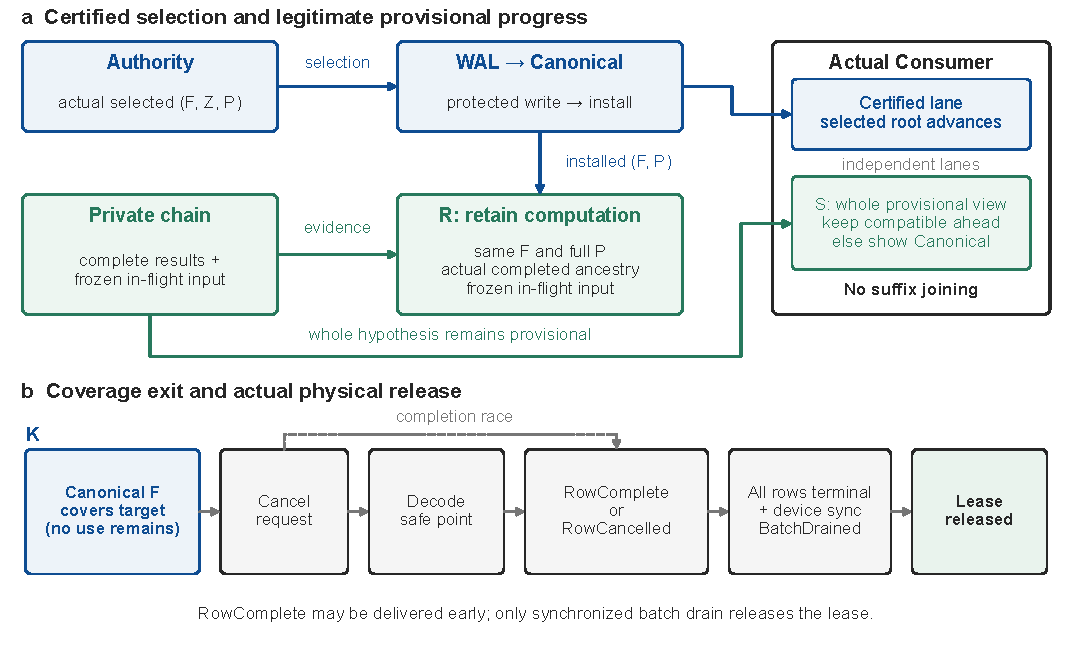
\includegraphics[width=\textwidth]{figures/coordination_protocol.pdf}
\caption{The core RevTrace runtime coordinates complete provisional computation and whole
Consumer views with certified state. $R$ and $S$ use the same declared
feedback dependencies, with separate sufficient guards. Coverage retirement
uses a different predicate. A complete result may be consumed before its
batch drains; only terminal rows plus device synchronization release the
physical lease.}
\label{fig:protocol}
\end{figure*}

\subsection{Complete results and physical ownership}
In the core runtime of Figure~\ref{fig:protocol}, dispatch binds session,
incarnation, job, input, target, and contract. A row returns either a
complete result with re-derived state/text or cancellation without partial
state. Complete rows can be installed and consumed before their batch
finishes. Only all terminal rows and device synchronization authorize
\texttt{BatchDrained} and executor reuse. The native process lifecycle
below has separate evidence.

\subsection{Covered work and safe-point exit: \texorpdfstring{$K$}{K}}
For the tested use model, $K$ requests exit when the installed Canonical
frontier covers a proposal's target and it has no remaining declared use.
This differs from $R$: valid work beyond the new root can remain useful.
Workers observe \texttt{CancelRequest} at decode boundaries; completion
can win, but each row has one terminal outcome. Static batches are not
compacted or refilled; masked costs and drain delays remain measured.

\subsection{Durable facts and outstanding input}
Before acknowledgment, synchronized frames bind parent/next states,
request identity, selected complete result, and receipt; recorded deltas
must reconstruct the state. Group-ready commit shares synchronization
among validated sessions without a collection timeout or cross-session
atomic transaction. Uncertain append/application outcomes block writes.
Write-ahead recovery~\cite{mohan1992aries} reconstructs facts and identities;
the native extension binds this to original correction calls.

\subsection{Validation boundaries}
Propositions~\ref{prop:rebase} and~\ref{prop:continuity} concern the stated
guards and compatible applications. The artifact retains an earlier,
separately frozen recovery prototype and its bounded model and crash
results; they do not validate the later core or native fault paths.
The selected-trace argument of Proposition~\ref{prop:refinement}, its
finite specification, and actual execution checks have distinct scopes.

% Integrated method extension; formal paired evaluation remains separate.
% Code hooks and evidence tiers are mapped in REVISION_BLUEPRINT.zh.md.
% Formal paired results remain pending; do not substitute six development trials.
\subsection{Continuing through delivery and process failures}
\label{subsec:native_resilience}
Each job has an Owner namespace and monotonic issue number; each physical
slot has a worker incarnation, following established RPC identity and
duplicate-suppression principles~\cite{birrell1984rpc}.
Fencing an incarnation removes message
authority without renaming its already accepted complete results.

\paragraph{Local rejection and physical release}
The ingress guard classifies events before changing busy slots or selected
state. Exact duplicates and fenced messages are local rejections that
cannot release newer leases. Contradictory currently owned contents freeze
writes; unknown exceptions remain failures. Per-incarnation Pipe endpoints
and receiver threads isolate incomplete logical frames from the Owner
loop. Replacement requires process exit, CUDA release, joined receivers,
and strict validation of complete receipts on the sealed channel. The
Owner then fences the incarnation and retires unfinished work. Accepted
complete buffers and supported whole views survive producer death with
their original identities.

\paragraph{Durable selection and recovery}
Before installation, a synchronous hook records complete parent/next
states, original correction and IDs, job identity, Owner/session epochs,
and producer incarnation. Framing, checksums, and chaining bind the fact;
synchronization precedes installation and publication. Uncertain writes
freeze the writer. Recovery may discard only an incomplete final frame;
complete corruption fails. These conventional write-ahead rules
\cite{mohan1992aries} bind the original feedback transition.

The surviving Supervisor continues the input ledger and original clocks
under the failure boundary of Section~\ref{sec:contract}. After confirming
old physical ownership has ended, it advances the Owner namespace,
replays the checked fact prefix, and cold-starts workers. Replay adds no
inference; old publications gain no new authority. Surviving provisional
views remain subject to subsequent root checks. Both schedulers share
this coordinator, durability, recovery, and actual Consumer; only
conditional full-call dispatch and retention differ.

% Preserve the existing label as a prose anchor, not a liveness theorem.
\paragraph{Conditional continued service}
\phantomsection
\label{prop:continued_service}
For finite accepted work after a finite supported failure prefix,
progress requires readable durable storage, eventual physical release
and loading, terminating original calls that advance pending frontiers,
fair Owner/Consumer scheduling, and unexpired recovery/service budgets.
Under these conditions, calls from the actual cut can discharge remaining
obligations without accepting fenced messages. This gives no RTO or
D2/C8 bound or unbounded liveness proof: cold loading, recovery, and
recomputation remain measured against original clocks.

\paragraph{Control history}
Current roots and live-call, complete-buffer, visible-view, and outbox
dependencies remain pinned. Actual Consumer acknowledgment releases
publication references, while the visible view stays pinned. Namespace
and issue high watermarks prevent ID reuse after collection. Unreferenced
terminal fingerprints and audit windows have fixed limits; full
diagnostics stream to disk. These are protocol-entry bounds relative to
active dependencies, not constant total memory: immutable input, current
state, cumulative text, and offline analysis remain separate.


\section{Evaluation}\label{sec:eval}
\subsection{Experimental design and service endpoints}
We evaluate two service obligations under unchanged selected feedback
histories: retaining dependency-valid progress already at the Consumer,
and completing selected transitions before their original deadlines.
The core factorial study isolates computation and whole-view retention;
the native study tests input-confirmed full execution of the original
correction pipeline. Timing, content support, and energy remain separate.
The core experiments use actual neural
calls, durable input and Canonical journals, and an instrumented FIFO
Consumer. Measurements use Consumer applications rather than publication
or display replay. Accepted input obligations retain
their original arrival clocks.

\paragraph{Implementation and workloads}
The service uses two 24-GB RTX~3090s: an FP16 Private worker and an FP32
Authority worker. Qwen3-ASR~1.7B~\cite{shi2026qwen3asr} is the primary backend; Whisper base.en~\cite{radford2023whisper}
tests a second adapter. The common carrier uses complete-row delivery,
at most 16 rows per batch, a 256-token generation limit, the protocol
kernel, and synchronized journals. These experiments use
\texttt{row\_complete}: physical early exit is disabled, so the effects of
$R$ and $S$ cannot be attributed to cancellation. Model startup is outside
the serving interval and is recorded separately. Serving energy integrates
both physical boards; CPU energy is outside that measurement.

The independent confirmation comprises 24 previously unused speaker
streams from LibriSpeech~\cite{panayotov2015librispeech}, totaling
714.11~s, selected using metadata before inference and partitioned into
three eight-speaker cohorts. Its 110 cells contain 60 primary cells
(three cohorts, two backends, two arrival patterns, five arms), 20
fresh-process repeat cells on cohort~A, and 30 coarser-feedback controls.
Primary Authority advances at every 2-s input boundary ($\rho=1$);
$\rho=3$ changes both selection frequency and feedback segmentation.
Synchronized streams start together; staggered streams start 0.25~s
apart. Repeats and arms reuse these sources: the independent acoustic
sample is 24 speakers, not 110 deployments.

\paragraph{Comparators}
The four arms cross computation retention $R$ with whole-view retention
$S$ (Section~\ref{sec:continuation}). With $R$ disabled, computation
rebuilds from the selected root rather than retaining its witnessed
continuation. With $S$ disabled, a Canonical application replaces the
provisional view with the new certified snapshot. This
\emph{checked-snapshot} Consumer still validates Private dependencies
against the same root and passes the same protocol kernel. Removing
retention does not remove validation, durability, input accounting, or
the execution capability of Section~\ref{sec:protocol}.
The fifth arm, \emph{Full composition (ours)}, is a complete-composition
positive control: an alternative policy instantiation with the same
retention relation, Consumer protection, and shared execution/commit
substrate. It is neither an external pre-existing implementation of our
complete design nor an independently reimplemented neural stack.
Comparable behavior is the expected positive-control outcome.

\paragraph{Endpoints}
For offered interval $i$, let $w_i$ be its audio duration, $r_i$ its
original ready time, $d_i$ its first actual visible covering time, and
$c_i$ its first actual certified covering time. Original joint-deadline
credit is
\begin{equation}
 A_{2,8}=\sum_i w_i\,\mathbf{1}
 \{d_i-r_i\leq2\ \land\ c_i-r_i\leq8\}.
 \label{eq:credit}
\end{equation}
All offered audio, including end-of-stream (EOS) tails and misses, stays
in its denominator. Whole-run service passes only when display P99 is
at most 2~s and certified-view P99 at most 8~s. P99 is computed over
offered frontiers within each run; credit weights their audio durations.
Thus a P99 pass can coexist with a small tail miss. We separately measure
adjacent visible-frontier withdrawals, their audio magnitude, and the
integral of the deficit below the previously observed high watermark.
Text revisions, final word error rate (WER), and board energy remain
separate endpoints. Independent recounters check complete selected
$F/Z/P/\mathrm{text}$ histories and reconstruct dependency witnesses from
actual complete outputs and consumed inputs, rather than trusting a
retention flag.

\subsection{Independent confirmation of the composition}
Table~\ref{tab:core-h3} reports the pre-specified Qwen, $\rho=1$,
staggered stratum, including all three cohorts. Retaining computation
alone raises deadline credit from 654.115 to 664.150~s but increases
audio-frontier withdrawals from 12 to 17. The additional work survives
the new root, while snapshot consumption still discards its visible
progress. Retaining views alone reduces withdrawals to one but yields
628.435~s of credit. The joint arm obtains 680.760~s and zero
audio-frontier withdrawals: 26.645~s, or 3.73 percentage points of offered
audio, above $R_0S_0$. Its gain over computation-only
is 16.610~s.

\begin{table}[t]
\centering
\caption{Independent Qwen confirmation, $\rho=1$, staggered arrivals.
Each arm offers 714.11~s across three eight-speaker cohorts.
Withdrawals and credit are totals; P99 and energy are medians of three
per-run statistics. All 15 runs miss the whole-run D2 criterion.}
\label{tab:core-h3}
\begingroup
\small
\setlength{\tabcolsep}{3pt}
\begin{tabular}{@{}lrrrr@{}}
\toprule
Arm & \shortstack{Audio\\withdrawals} &
\shortstack{Display\\P99 (s)} & \shortstack{D2/C8\\credit (s)} &
\shortstack{Energy\\(J/audio-s)}\\
\midrule
$R_0S_0$ & 12 & 3.797 & 654.115 & 59.72\\
$R_0S_1$ & 1 & 3.891 & 628.435 & 59.16\\
$R_1S_0$ & 17 & 2.431 & 664.150 & 59.68\\
$R_1S_1$ & 0 & 2.329 & 680.760 & 59.37\\
Full (ours) & 0 & 2.534 & 667.530 & 59.73\\
\bottomrule
\end{tabular}
\endgroup
\end{table}

The cohort-wise credit interaction,
$I=Y_{11}-Y_{10}-Y_{01}+Y_{00}$, is
$+18.530$, $+6.205$, and $+17.555$~s. These three contrasts share queues
within each cohort. They support a composition effect
in this stratum, rather than treating individual deadline windows as
independent trials. The joint arm still erases 569 visible characters:
zero audio-frontier withdrawal does not mean immutable text.
Its 2.329-s median display P99 also remains above D2. The result preserves
more timely progress without establishing that this workload meets its
whole-run service target.

The full composition likewise has zero frontier withdrawals, the same 569
erased characters, and comparable timing and energy. Its lower credit
than the joint arm in this stratum is not evidence that a different
complete composition is inherently inferior. Across the confirmation,
all 144 matched source/backend/granularity/arrival history groups agree
on complete Canonical $F/Z/P/\mathrm{text}$; all 22 paired full-composition
comparisons preserve those histories. The ablations therefore isolate
how legal progress is retained, rather than buying latency by changing
the selected feedback task.

\subsection{Relative progress explains when retention matters}
The useful opportunity is an already observed whole view ahead of a
new Canonical frontier whose complete dependency path remains valid.
In the headline joint arm, 18 of 368 Canonical updates encounter such
a view and retain it. Computation-only encounters 17 and clears all 17.
Under synchronized arrivals the joint arm encounters only three of
368; its credit is 0.790~s below computation-only. Without an ahead
view, preserving it has little service value. These are witnessed
incidences in the executed workload, not a production prevalence estimate.

Timing can also change the ranking. In the fresh-process staggered
repeat on cohort~A, joint credit is 226.320~s versus 230.565~s for
computation-only, and $I=-2.245$~s. We retain this repeat alongside
the three positive primary contrasts. The combination's value depends
on relative progress and actual feedback compatibility; independent
source confirmation does not imply an invariant timing advantage.

\subsection{Operating workloads and subsequent timely continuity}
We next freeze three development workloads---eight synchronized
sessions, eight staggered sessions, and sixteen staggered sessions---with
four arms and three fresh processes per arm (36 cells). A single later
exploratory midpoint adds twelve staggered sessions and the same twelve
arm/repeat cells. Figure~\ref{fig:service-region} retains all 48 runs.
The nested source lists offer 121.205, 185.300, and 250.180~s per
eight-, twelve-, and sixteen-session run. Adding sessions also adds
source content; these are explicit operating workloads, not a pure
concurrency capacity curve.

\begin{figure*}[t]
\centering
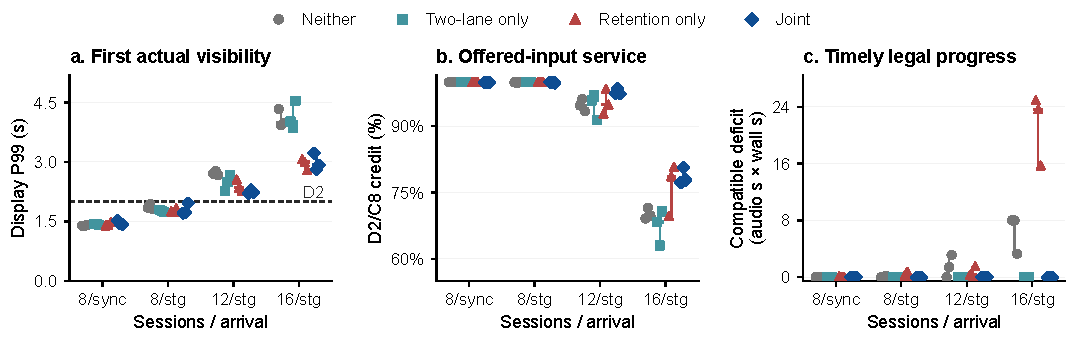
\includegraphics[width=\textwidth]{figures/service_region.pdf}
\caption{All four development workloads and three fresh-process runs per
arm, including the negative twelve-session midpoint. Points are real
per-run values; ticks and ranges describe their median and observed
range. Panel~(c) is the separate secondary measure of subsequent
compatible loss of originally timely intervals, censored at the next
Canonical root when necessary. It does not replace panel~(b)'s original
first-observation credit.}
\label{fig:service-region}
\end{figure*}

All arms pass whole-run D2/C8 in the two eight-session workloads.
Joint display P99 is 1.426--1.528~s when synchronized, where the arms
largely converge. Staggered joint P99 reaches 1.955~s, and an earlier
development run reached 2.034~s, exposing a narrow timing margin.
Two 0.215-s tails exceed D2 in the new eight-session runs and remain
uncredited even though their runs' P99 passes. At sixteen sessions,
all twelve runs fail D2, while C8 passes. Joint credit exceeds $R_0S_0$
by 20.280/22.885/20.180~s, but its credit interactions are
$+20.910$, $+26.380$, and $-9.575$~s.
Against computation-only, joint credit changes by
$+18.910$, $+5.055$, and $-7.225$~s, and display P99 improves
in only one repeat. Continuity is the stable distinction: computation-only
withdraws compatible views 16/17/12 times, versus zero for joint.

First credit does not reveal a later withdrawal. A frozen secondary
recount therefore follows intervals already delivered within D2 whose
eventual certified covering view also meets C8. At each subsequent
Canonical application it classifies withdrawal using the complete old
view's dependency witness, separately recording necessary incompatible
withdrawals. Loss lasts until an actual covering view returns or the
next Canonical boundary censors this root's window. At sixteen sessions,
computation-only still has 10/12/9 timely compatible loss windows with
24.903/23.635/15.736 audio-s$\times$wall-s deficit area; joint has none.
Such holes intersect the original D2 read point for 6.000/10.675/4.000~s
of distinct audio. The secondary measures continuity after delivery;
it neither changes Eq.~\eqref{eq:credit} nor certifies provisional content.

The twelve-session witness is \emph{not established}: all twelve runs
fail D2, and computation-only never loses a timely complete non-EOS
interval satisfying the frozen witness criterion. Joint has no compatible
loss windows. The predeclared stop rule ends this search; full criteria
and per-run results remain in the artifact.

\subsection{Quality and cost boundaries}
All headline Qwen arms have WER $26/1908=1.36\%$ and identical selected
histories. Retrospective support counting first-certified content plus
first-ahead whole views that exactly match later same-$F$ Canonical
text leaves the headline credits unchanged. Elsewhere raw differences
remain: joint loses 2~s of strict support in the sixteen-session third
repeat and 2~s in each of the midpoint's first two repeats, although
the frozen text normalizer agrees. This comparison is with the selected
model output, not human-transcription correctness. Whisper exposes a
larger adapter boundary: WER is 83.12\% at $\rho=1$ and 11.53\% at
$\rho=3$, whose different feedback contract prevents interpreting it
as a quality-preserving speedup.

The headline arms consume similar board energy (Table~\ref{tab:core-h3});
energy does not rank them in credit order. At sixteen development
sessions, joint reduces total model time by 0.66--1.59~s against $R_0S_0$,
while serving wall time does not consistently fall and the
three energy differences change sign. The measured benefit is the
progress delivered and preserved under a fixed feedback contract.
It is not a general reduction in inference cost or a cure for overload.

% Complete service evidence; component, development and independent scopes stay separate.
% All service numbers here retain their actual pre-resilience NN source:
% bdfa3b1307d267a5a4caf6484e1ad465c39a592e. They are not relabelled as 4f4c3c.
\subsection{Native correction with the original selected task}
\label{subsec:native_retention_eval}
We retain StreamCorrect's published recognizer, learned correction, and
feedback update~\cite{vu2026streamcorrect}, using the fixed 500-ms, no-VAD
adaptation and original FP32 execution. Both compared policies have two
protected full workers, the same ASR early-view Consumer, and identical
neural warmup. Conservative execution waits for selected parent feedback
before starting the next call; full-call retention confirms conditional
calls as in Section~\ref{subsec:native_full_calls}.
We distinguish the earlier frozen native implementation (\texttt{bdfa3b13})
from the resilience implementation (\texttt{4f4c3cab}). Historical independent
confirmation and the new matched comparison retain their own identities.

\paragraph{Development and frozen confirmation}
Development on AISHELL-1~\cite{bu2017aishell} tests original full and
buffer-only steps, including projected ends that differ from selection
without invalidating their inputs. Full calls, unlike ready-only ASR
handoff, retain still-executing work. The artifact retains the pilot and
development matrix, including two 0.068-s EOS misses.

For the earlier \texttt{bdfa} independent confirmation, the method was
frozen before metadata selection of four unused AISHELL-1 speakers in
an 8--9-s band; all initial selections remain. Two policies
and two fresh-process repeats give 16 runs, with randomized pair blocks,
reversed arm order, and swapped GPU roles. Speakers are the independent
acoustic units. Every original 500-ms frontier and partial EOS stays in
the denominator.

\paragraph{Task fidelity and timely service}
Offline original full calls supply 68 reference transitions, separately
from service timing. All 272 Canonical transitions in this confirmation reproduce
their complete original start and end states, $C$, and returned IDs,
including the implementation tag. Both arms have five character edits
over 81 unique reference characters, or 6.17\% CER. This measures the
adaptation, not the published author's benchmark CER.

\begin{table}[t]
\centering
\caption{Matched version comparison: four previously measured speakers,
two policies, two versions, and two fresh trials (32 runs).
Each row offers 66.340~s. Credit and board energy are totals;
D99 is the median of per-run values. Energy uses one common external
origin-to-confirmed-physical-model-drain window, an upper observation
bound. This is a matched regression study, not new acoustic confirmation.}
\label{tab:native_full_confirm}
\small
\setlength{\tabcolsep}{2.5pt}
\begin{tabular}{@{}llrrrr@{}}
\toprule
Version & Policy & \shortstack{Credit\\(s)} & \shortstack{D99\\(s)} &
\shortstack{Energy\\(kJ)} & Pass\\
\midrule
\texttt{bdfa} & Conserv. & 33.500 & 4.450 & 44.690 & 0/8\\
\texttt{bdfa} & Full-call & 66.340 & 1.633 & 39.735 & 8/8\\
\texttt{4f} & Conserv. & 30.000 & 4.759 & 47.019 & 0/8\\
\texttt{4f} & Full-call & 65.822 & 1.638 & 43.952 & 6/8\\
\bottomrule
\end{tabular}
\end{table}

The earlier independent confirmation on \texttt{bdfa} raises credit from
37.0 to all 66.33975~s and whole-run passes from 0/8 to 8/8.
We then freeze a matched 32-run comparison on those same four sources,
with common FP32 models, neural warmup, allocator, swapped GPU roles,
and external board-power observation. All 544 selected transitions
reproduce complete original inputs/outputs, $C$, and IDs under the
declared static code-version mapping. Table~\ref{tab:native_full_confirm}
reports these new runs. The final implementation raises credit from
30.0 to 65.821625~s and passes from 0/8 to 6/8. Its two failures are
S0908 EOS intervals: paired display P99 increases by 0.163/0.050~s
against \texttt{bdfa}. Other paired differences have both signs;
similar medians do not establish equivalence. Through confirmed physical
model drain, final Full-call uses 6.52\% less board energy than final
Conservative and 10.61\% more than earlier Full-call. Model drain and
source-specific service cleanup have different endpoints; separate
EOS-window and original per-version results remain in the artifact.

\paragraph{Resident independent requests}
A new finite contract keeps the models and workers resident while a
single client submits four pre-registered, independent requests. Each
original file EOS closes its request; the next origin is assigned only
after actual certified EOS consumption. This is closed-loop request
service, not online VAD, one continuous recording, or open-arrival
capacity. Two policies and two fresh trials preserve all 272 original
transitions and per-request input clocks. Both worker PIDs persist across
each trial's requests, with one initial model load. Full-call meets D2/C8
on 7/8 requests versus 0/8, earning 64.118875 versus 31.0 of 66.33975~s
offered. The second repeat's S0908 request has D99 2.229~s; residency
does not establish an invariant deadline margin.

\paragraph{Retained work and visible content}
The earlier independent confirmation contains 92 promoted calls whose
recognition begins before their selected parent finishes; 20 have their
own predicted end differ from original correction. Twenty-four invalid
or covered calls stop after ASR, and two completed wrong-input results
are discarded, without changing selection. This separates input
confirmation from requiring correct future predictions.

One original-source Canonical update from 4.0 to 4.5~s keeps a supported
5.0-s view and its executing call. Two necessary updates withdraw 6.0 to
5.5~s when the actual parent refutes the complete input. These witnessed
cases do not estimate another $R\times S$ interaction or natural rate.

In that earlier confirmation, first whole-text agreement with later
same-$G$ Canonical text supports 29.0 versus 51.518125~s of credited audio;
14.821625~s of Full-call credit lacks support, with zero unknown coverage.
Raw and whitespace-only comparisons agree. Unchanged-text rows cover
10.0 versus 17.0 credited seconds. Frontier credit is neither newly
transcribed characters nor human correctness.

An earlier two-source capacity comparison remains negative: retention
earns 17.0~s versus 18.5~s for independent full replicas, at higher energy
and with a different warmup/Consumer. Single-chain gains do not establish
superior saturated multi-source capacity.

\subsection{One coordinator through faults and sustained state}
\label{subsec:same_source_validation}
The failure and state study uses \texttt{4f4c3cab}, the resilience version
also compared in Table~\ref{tab:native_full_confirm}, with separately
frozen workloads. Both policies share durability,
message guards, recovery, Consumer, original FP32 models, and the
\texttt{expandable\_segments:True} allocator setting. Initial loading and
fixed warmup precede the serving clock; replacement loading, replay,
recomputation, and final physical drain remain inside it.

The short bank has six conditions, two policies, and two fresh processes
on one development clip (24 trials), plus four EOS/compatible-view
regressions. Across these and eight sustained trials, an independent
checker binds all 3,976 durable selected transitions to original complete
call receipts and actual Consumer applications. It finds no illegal
installation or incorrect owned-message rejection, and preserves every
accepted input and its original clock. Eight injected duplicate/late
messages are locally rejected without Canonical mutation; eight
worker-only deaths have confirmed physical replacements. Short reference
comparisons map only the static code-version tag; long comparisons are
unprojected. Conditional calls contribute 354 durable facts; 352 have
an original Owner installation record, and two first reach the Consumer
through recovery. There is no completed-buffer installation in these trials.
In four worker-after-ASR cases, an already consumed whole view remains
in Consumer state across its producer's exit and fencing until legitimate
Canonical correction. This is retained availability, not another delivery
of the old job or a claim that its prediction was correct.

\begin{table*}[t]
\centering
\caption{Same-source short fault study: six conditions on the fixed
development clip, two fresh trials per policy. Each cell lists
Conservative above Full-call; ranges are observed minima and maxima,
not confidence intervals. Illegal; done gives illegal installations and
completed/2 trials. Reject/mutation counts local rejections and resulting
Canonical changes. New result measures fault to actual certified
consumption of a new durable fact whose original call completes after
the fault; it excludes old-fact replay and replacement readiness.
D2/C8 counts joint whole-run passes; EOS counts D2 misses. Both-board
energy spans the original serving clock through physical drain.}
\label{tab:native_reliability}
\begingroup
\fontsize{8.5}{10}\selectfont
\setlength{\tabcolsep}{3pt}
\begin{tabular}{lrrrrrr}
\toprule
Condition & Illegal; done & Reject / mutation & New result (s) & D2/C8 pass & EOS miss & Energy (J) \\
\midrule
No fault & \shortstack{0; 2/2\\0; 2/2} & \shortstack{0 / 0\\0 / 0} & \shortstack{--\\--} & \shortstack{0/2\\1/2} & \shortstack{2\\1} & \shortstack{6566--6574\\5896--5911} \\
Duplicate / late & \shortstack{0; 2/2\\0; 2/2} & \shortstack{4 / 0\\4 / 0} & \shortstack{--\\--} & \shortstack{0/2\\1/2} & \shortstack{2\\1} & \shortstack{5701--5893\\5538--5846} \\
Worker after ASR & \shortstack{0; 2/2\\0; 2/2} & \shortstack{0 / 0\\0 / 0} & \shortstack{1.90--2.22\\2.15--2.21} & \shortstack{0/2\\0/2} & \shortstack{2\\2} & \shortstack{5182--5401\\5447--5647} \\
Worker partial frame & \shortstack{0; 2/2\\0; 2/2} & \shortstack{0 / 0\\0 / 0} & \shortstack{2.10--2.25\\1.76--2.23} & \shortstack{0/2\\0/2} & \shortstack{2\\2} & \shortstack{4775--5178\\5492--5594} \\
Owner before durable & \shortstack{0; 2/2\\0; 2/2} & \shortstack{0 / 0\\0 / 0} & \shortstack{86.42--108.08\\64.61--107.09} & \shortstack{0/2\\0/2} & \shortstack{2\\2} & \shortstack{24549--28019\\19571--26557} \\
Owner after durable & \shortstack{0; 2/2\\0; 2/2} & \shortstack{0 / 0\\0 / 0} & \shortstack{83.90--87.05\\101.80--104.44} & \shortstack{0/2\\0/2} & \shortstack{2\\2} & \shortstack{22415--24200\\26483--27171} \\
\bottomrule
\end{tabular}
% Fixed vertical order within each cell: Conservative / Full-call. Ranges are two fresh trials, not confidence intervals.
% New result copies frozen 4f fault_to_new_certified_result (runtime model_end>=fault filter). Any strict > statement is a separately audited observed property.
% A qualifying call may already be in flight on a surviving worker. This clock is neither replacement-neural readiness nor old durable replay.
% Illegal installs require independent trace-checker evidence. ? means unknown. -- means not applicable, not zero.
% Main table: development S0908 24 cells only. Regression4 and sustained8 remain separately listed in ALL36_MACHINE_TABLE.

\endgroup
\end{table*}

Table~\ref{tab:native_reliability} retains deadline failures. Normal
Full-call display P99 is 1.798--2.053~s: one of two fresh trials passes,
while the other misses D2 only at EOS. Duplicate/late delivery has the
same one-of-two boundary. All worker-fault trials fail D2 but pass C8;
all Owner-fault trials fail both. After durable selection, old facts
reappear in 1.36--1.81~s, whereas new certified post-fault completions
take 64.61--108.08~s across the Owner cases. A surviving worker can
provide a post-fault completion before replacement readiness. Neither
replaying a fact nor finishing the task establishes fault-time D2/C8.

\paragraph{Complete results across producer death}
The 36 trials do not install a completed conditional buffer. We therefore
freeze two matching-input and two mismatching-input timing cases on a
development source. A transport fixture holds the parent after original
ASR and the child after sending its complete original result. After
the Owner registers that result, we kill its producer, check actual
exit, CUDA release, sealed-channel validation and incarnation fencing,
then release the parent's original correction. All four executions
complete their protected task. Independent reconstruction confirms that
both matching cases install and consume the original result once,
preserving its job, birth and incarnation; both mismatching cases reject
it using the actual same-frontier parent input. The positive cases also
complete a subsequent independent request. These are controlled
interleavings, not natural incidence or fault-time SLO evidence.
A separately frozen, zero-NN reconstruction validates these unchanged
runs; their original audit gates remain failed and are retained in the
artifact with the READY indexing defect.

\paragraph{Controlled sustained-state stress}
Two metadata-selected AISHELL-1 speakers supply 24 utterances each,
concatenated as exact PCM into 228.51025-s and 208.1003125-s synthetic
streams without resets or EOS at joins. A continuous original-engine
reference without between-step restoration and 875 separately restored
steps agree on complete start/end state, $C$, and IDs, crossing 398/357
actual buffer shifts and 353/252 context changes. Two policies and two
fresh processes yield eight trials and 3,500 matching selected steps.
Unpinned terminal receipts and each retained audit class stay at or
below 64 entries; live dependencies, serialized state/output, Owner RSS,
and cumulative disk logs remain separate.

This is state stress, not viable continuous ASR: all eight trials fail
D2/C8, with display P99 of 449.727--502.952~s. Both policies reproduce
the original task's severe insertion errors: CER is 3103/486 (638.48\%)
and 1313/522 (251.53\%) on the two streams. Full-call also uses more
board energy. The original decoder's length guard can skip its decoding
loop, so frontier credit need not add decoded text. The checker observes
90 compatible-ahead applications, all preserved, and 1,118 necessary
incompatible withdrawals across the 36 trials. These are controlled
coverage counts, not natural prevalence or transcription correctness.
\paragraph{Input confirmation and actual use}
A separate read-only audit pairs all 5,529 actual dispatches with the
selected complete cut at their start frontiers. Of 1,901 conditional
dispatches, 360 inputs eventually match, 1,541 are refuted, and none
remain unresolved. Matches are 40/57 on normal short traces, 58/90 under
controlled faults, and 96/924 and 166/830 on the two no-reset sources.
These strata have different workloads and acoustic units; their pooled
ratio is not a production estimate. Six matched conditional jobs fail
to become durable after injected process failures. Thus eventual input
equality, live ownership, durable selection, installation, and actual
consumption require separate accounting.

Own predicted-end disagreements (409/457 and 333/416 observed predictions)
are selected-call diagnostics, not the dispatched-input denominators.
The first observed D2/C8 misses and a conservative offline excess-length
bound both precede the after-trim 448-token condition on each stream.
The length bound allows all reference characters in the currently started
utterance, including future ones. It is neither online prefix CER nor a
reset signal, and the observations do not identify a unique causal mechanism.

% Compressed earlier K24 support; full measured ledger remains in the artifact.
% This core execution evidence is separate from native failure validation.
\subsection{From physical release to supported service}
\label{subsec:release_evidence}
A separate 24-run core study crosses $R$ and $K$ with $S$ enabled,
two arrival patterns and three fresh processes, using a frozen
wrong-conditioning fixture. Selected histories and WER $14/687$ match;
all 675 same-input/prompt/audio/peer-order pairs return identical outputs.
Synchronized $R1$ releases the next 16-row computation 473--577\,ms
earlier. All 96 following rows are actually consumed and their whole
texts match later same-frontier Canonical text. Only 6/6/1 rows switch
from deadline miss to hit. Adding $K$ changes credit by +7.970 to
+15.255\,s when synchronized and $-26.000$ to $+21.780$\,s when
staggered, without consistent energy savings. Request acknowledgment
still precedes physical drain. This is a measured release-to-service
opportunity, with no stable positive $R\times K$ interaction.


\section{Related Work}\label{sec:related}
\paragraph{Incremental information and dependency reuse}
The incremental-unit model separates newest committed information from
the active right edge and propagates dependency revocation
\cite{schlangen2011incremental}. Its commit promises that a unit will not
be revoked. Here, certification records acceptance by the protected
selection protocol; later selected facts may still revise the transcript.
Adapton checks recorded dependencies; Nominal Adapton combines names with
arguments and dependency checks to recover reusable work
\cite{hammer2014adapton,hammer2015names}. Differential Dataflow maintains
incremental computations across evolving versions
\cite{mcsherry2013differential}. These works establish much of the basis for
dependency-aware reuse. RevTrace instantiates that basis for complete
neural feedback state and frozen executed calls. Its service obligation
connects execution eligibility to the actual whole view retained when an
independently selected root is applied.
Our sufficient witness follows recorded executions; it does not transfer a
from-scratch theorem to independently repeated floating-point inference.

\paragraph{Revisable speech services and speculation}
Whisper-Streaming converts an offline recognizer into incremental service
using LocalAgreement~\cite{machacek2023whisperstreaming}. StreamCorrect
adds learned correction and feeds selected corrections into subsequent
recognition~\cite{vu2026streamcorrect}. RevTrace retains that selection and
feedback behavior in its controlled native adapter; its contribution
concerns the asynchronous execution and consumption around the feedback
boundary. It does not introduce a better acoustic model or train a new
corrector.

SSBD coordinates old-output draft reuse with display-only suffix masking
\cite{zeng2026ssbd}. It revalidates a draft under updated input and includes
an unbiased configuration. RevTrace follows complete calls that actually
executed to establish their eligibility under newly selected feedback state,
then checks the dependency witness for the Consumer's whole current view.
PredGen provides a close precedent for speculation while speech input
evolves across recognition, language generation, and speech synthesis
\cite{li2025predgen}. Our comparison holds the complete selected feedback
task fixed across the retention policies. The specific reuse object,
protected selection, and whole-view transition define the composition
evaluated here. RelayS2S uses a learned verifier to commit a fast-path
prefix that constrains subsequent slow-path generation
\cite{mai2026relays2s}. Our native calls instead confirm their complete
inputs and retain the original correction and feedback update. Work on
ASR alignment drift also establishes the importance and cost of audio
position state~\cite{wang2026alignmentdrift}; our contract includes that
state rather than treating text equality as sufficient.

\paragraph{Execution, authorization, and recovery}
Retire studies versioned execution and bounded physical exit for
interruptible agents~\cite{zhang2026retire}. RevTrace likewise distinguishes
logical progress from an executor's actual release, while deriving the
tested retention and coverage decisions from the feedback contract. Our
simple covered-exit implementation is execution support, without a claim
to a new general cancellation algorithm. A parent-version cancellation
control is not a reproduction of the complete Retire system.

Optimistic and multiversion concurrency control separate validation and
commit from concurrent execution~\cite{kung1981occ,bernstein1983mvcc}.
Write-ahead recovery persists state changes and identities
\cite{mohan1992aries}, and stream-processing systems coordinate recoverable
state~\cite{carbone2017flinkstate}. We use these established principles at
the ASR feedback boundary. They supply machinery for ordering and
durability; the adapter still has to specify which state constitutes a
valid continuation and which complete view the Consumer may retain.

\section{Discussion}\label{sec:discussion}
\paragraph{Scope of the guarantee}
The continuation witness assumes a sufficient adapter state and faithful
execution of frozen inputs. A new adapter must account for every mutable
field that can affect later inference, selection, or feedback. A hidden
KV cache, alignment cursor, or external tool state can invalidate a
token-only argument. Conservative rejection remains allowed when a
sufficient witness is absent. The guarantee concerns dependency validity
and an individual compatible application; it supplies neither transcription
correctness nor monotone text for an entire session.

\paragraph{Progress, content, and capacity}
Processing more audio can leave the cumulative transcript unchanged.
Frontier credit, actual text additions and revisions, eventual selected
text agreement, and ground-truth accuracy answer different questions. We
report them with their original denominators. Preserving compatible
progress also cannot remove all input synchronization, queueing, or neural
work. The negative c12 witness and the native two-replica comparison
identify concrete limits of this implementation rather than a universal
capacity envelope. The independent native confirmation establishes a
single-chain service opportunity with the original selected task; it
does not turn that result into saturated multi-source capacity.

\paragraph{Deployment and validation}
The continuous-original reference exercises the native cut across real
buffer and context changes; another adapter must establish its own state
sufficiency. Active-dependency collection bounds protocol entries relative
to live references, separately from cumulative text, current state, and
total memory. Owner/worker recovery assumes the surviving services of
Section~\ref{sec:contract}. Replaying old facts restores access to that
prefix; the measured cold Owner restarts still miss original deadlines
for new work. Broader ownership transfer requires separate validation.
Finite specifications, source controls, controlled faults, actual GPU
service, and retrospective checks provide distinct evidence.

\paragraph{Eligibility and resource admission}
A valid input witness determines whether an owned call may be used.
It does not determine whether starting another conditional call is
worthwhile. Limiting new speculation can leave existing supported whole
views intact. The long stress study motivates this separate resource
decision. In a bounded two-client probe, new speculative calls precede
another client's ready necessary call in both repeats. The later client
has no additional C8 misses, and its C99 penalty fails the predeclared
repeat-consistency gate. No admission controller or general native-session
fairness is evaluated.

\section{Conclusion}\label{sec:conclusion}
RevTrace separates complete-input eligibility, original selection authority,
and whole-view support while trusted feedback advances. Service experiments
expose a coordination gap: first delivery can meet its deadline, yet a
compatible update can withdraw that progress. The joint design protects
the supported ahead view. Native full calls can retain original correction
work after their inputs are confirmed even when their own next predictions
are wrong. Durable facts and physical identities carry this distinction
through supported process failures. The resulting composition connects
dependency reuse to actual continued consumption under a fixed feedback
task, with measured timing, content, recovery, and capacity boundaries.
Extending recovery to Supervisor failure remains a separate direction.

\section*{AI Tool Usage}
ChatGPT/Codex assisted literature discovery, drafting and revision of all
manuscript sections and the refinement argument, runtime extensions and
experiment orchestration, and validation/analysis code producing the
figures and tables from recorded measurements. The artifact records
execution sources, frozen configurations, controls, and result provenance,
separating actual service measurements from component tests and
retrospective analyses. Constructed streams concatenate recorded AISHELL-1
PCM. The authors retain responsibility for the submission.
\clearpage
\bibliographystyle{IEEEtran}
\bibliography{refs,formal_refs,coordination_refs}
\end{document}
